\chapter{Método Proposto} \label{cap:metodoprop}
  
O método proposto se utiliza do GRASP, do ILS e da abordagem exata através da
programação linear inteira, pretendendo tirar proveito das vantagens de cada
uma dessas técnicas. Ou seja, combinando a agilidade dos métodos heurísticos com
a optimalidade do método exato.
  
Da mesma forma que em outras abordagens heurísticas, esse novo algoritmo
consome pouco tempo computacional, em relação ao método exato e tem a capacidade
de escapar de mínimos locais.
  
O GRASP foi utilizado como a base do algoritmo, onde a parte da construção
seguiu a sua definição padrão, com a geração de uma lista restrita de candidatos
(LRC) e a posterior escolha aleatória entre esses elementos. A parte da busca
local foi adaptada para executar em conjunto com o ILS modificado. Para o ILS
foram definidos algumas estruturas de vizinhança que foram utilizadas
na busca local, e a perturbação foi feita com a utilização de um \textit{solver}
em uma parte do problema. Essa abordagem permite que o algoritmo gere boas
soluções e escape de mínimos locais além de promover uma aceleração na obtenção
de boas soluções, pois quando o \textit{solver} encontra uma melhor solução ele
consegue mudar o espaço de soluções em que a busca era efetuada.


O \textit{solver} é utilizado para resolver um modelo matemático que foi
desenvolvido baseado na proposta de \cite{pontes2002} que é aplicado a uma parte do problema cada
vez que se deseja fazer uma perturbação. Enquanto a busca local usa o método de
descida, variando entre três estruturas de vizinhança, o \textit{swap-x}, o
\textit{crossover} e a \textit{compactação}. Mais adiante serão dado mais
detalhes sobre o modelo matemático, a forma de escolha do sub problema, da fase
de construção que foi implementada, da busca local e das implementações que não
tiveram êxito.

\section{Modelo matemático} \label{sec:modelomat}

   
A modelagem proposta por \cite{pontes2002} aborda todas as restrições do
problema fazendo com que a quantidade de restrições geradas seja muito elevada.
A idéia utilizada na nossa formulação é a de tentar reduzir ao máximo a
quantidade de restrições necessárias. Isso é feito com a modelagem de apenas
algumas restrições, aquelas que são possíveis no mundo real.

Primeiro se percebeu que não há necessidade de modelar os 4 tipos de arcos para
cada voo, uma vez que dados dois voos só pode vir a ocorrer dois tipos de arcos
possíveis entre eles. Essa situação é ilustrada na Figura
\ref{fig:modelagem_arcos}.

\begin{figure}[ht]
	\centering
	\caption{Arcos necessários para ligar dois voos. \newline \mbox{Fonte:
	(Própria)}}\label{fig:modelagem_arcos}
	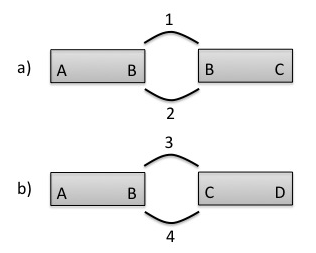
\includegraphics[scale=0.4]{./img/modelagem_arcos}
\end{figure}


Em a) os voos respeitam a restrição geográfica, dessa forma apenas os arcos de
tipo 1 e 2 precisam ser modelados uma vez que não teria sentido fazer um voo de
reposicionamento nessa situação. Em b) os aeroportos em questão são diferentes,
sendo necessário apenas a modelagem dos arcos do tipo 3 e 4, perceba que não
teria outra alternativa se não fazer um voo de reposicionamento.

\subsection{Definição}

Seja $D = (V,A)$ um grafo representando uma instância do PCTA, onde o conjunto
de vértice $V = {v_{i}:i \in I}$ de D é indexado por $I = {1, 2, ..., n+1,
n+2}$ onde $v_{n+1}$ e $v_{n+2}$, identificam, respectivamente, os nós fonte e
destino. E os nós restantes referem-se ao conjunto de nós originais, com $n$
elementos. Sejam os custos ${c_{ij}:(i,j) \in A}$ introduzidos acima, estando
associados com cada arco do grafo.
  
Seja ${x_{ij}:(i,j) \in A}$ um conjunto binário 0-1 de variáveis usada para
controlar a inclusão $(x_{ij} = 1)$ ou a exclusão $(x_{ij} = 0)$ de um arco
(possível conexão) entre vértices (voos) $v_{i}$ e $v_{j}$. O conjunto
$\overline{I}$ identifica o conjunto de nós excluindo o nó fonte $(v_{n+1})$ e
o nó de destino $(v_{n+2})$. A função objetivo foi dividida para facilitar o
entendimento de como é feito o custo de adicionar um trilho. Variáveis reais
$\delta_{i}$ e $\theta_{i}$, $i \in \overline{I}$ são usados para representar,
respectivamente, o desvio do tempo de partida sugerido e a norma desse desvio
para $v_{i}$. Essas variáveis devem no entanto obedecer $-\gamma_{i} \geq
\delta_{i} \geq \gamma_{i}$ e $0 \geq \theta_{i} \geq \gamma_{i}$, onde
$\gamma_{i}$ é o valor máximo de desvio permitido (em cada direção) do tempo de
partida sugerido para o voo. Finalmente o tempo de partida sugerido que é dado
por $s_{i}:i \in \overline{I}$.
  
\section{Função objetivo}

\begin{equation}
Minimizar \  \ \sum_{j \in \overline{I}} x_{v_{n+1}j}(CUSTO\_TRILHO) + \sum_{i \in
\overline{I}} \sum_{j \in I} x_{ij}c_{ij} + \sum_{i \in
\overline{I}} \theta_{i}
\end{equation}

\section{Restrições}

\begin{enumerate}


\item[a)] Garantia de recobrimento dos voos \\
\begin{equation}
  \sum_{i \in I} x_{ij}= 1 \   \ \forall_{j} \in \overline{I} 
\end{equation}
\begin{equation}
\sum_{j \in I} x_{ij} = 1 \   \ \forall_{i} \in \overline{I}
\end{equation}


\item[b)] Viabilidade das conexões \\
\begin{equation}
s_{i} + t_{i}x_{ij} - M(1 - x_{ij}) + \delta_{i} \leq s_{j} + \delta_{j} \   \ \forall_{i,j} \in \overline{I}
\end{equation}
%\begin{equation}
%\sum_{i \in I} x_{i(n+1)} = 0
%\end{equation}
%\begin{equation}
%\sum_{j \in I} x_{(n+2)j} = 0
%\end{equation}

\item[c)] Modulo do desvio do tempo de partida sugerido \\
\begin{equation}
\theta_{i} \geq \delta_{i} \   \ \forall_{i} \in \overline{I}
\end{equation}
\begin{equation}
\theta_{i} \geq -\delta_{i} \   \ \forall_{i} \in \overline{I}
\end{equation}

\item[d)] Limites das variáveis \\
\begin{equation}
0 \geq \theta_{i} \geq \gamma_{i} \   \ \forall{i} \in \overline{I}
\end{equation}
\begin{equation}
-\gamma_{i} \geq \delta_{i} \geq \gamma_{i} \   \ \forall_{i} \in \overline{I}
\end{equation}
\begin{equation}
x_{ij} \in \{0,1\}
\end{equation}
\end{enumerate}

\clearpage

A função 1 do modelo representa a função objetivo onde a primeira parte
representa o custo de inicializar um trilho, ou seja, sempre que um arco
partindo de $n+1$, que é o nó origem, for ativado acrescenta-se o custo de um
trilho a solução. A segunda parte representa o custo de adicionar os demais
arcos e a terceira parte representa a adição do módulo dos atrasos que foram
utilizados. Perceba que a primeira e a segunda parte podem ser modeladas juntas,
a sua separação foi feita para facilitar o entendimento do modelo.

As restrições 2 e 3 representam respectivamente que todos os nós deverão
ter apenas um antecessor e um sucessor, as únicas exceções são o nó origem que
pode incidir em vários outros nós e o nó de destino que pode ser incidido por
vários nós.

A restrição 4 é utilizada para manter a viabilidade das conexões acrescentando
atrasos a elas se for necessário. Se $x_{ij} = 1$ então tem-se que o tempo de
partida do voo i ($s_{i}$) mais a duração do voo do seu voo ($t_{i}$) mais um
possível atraso nesse voo ($\delta_{i}$) deve ser menor ou igual ao tempo de
partida do voo j ($s{j}$) mais um atraso que lhe seja dado ($\delta_{j}$). Se
$x_{ij} = 0$ então M irá validar automáticamente essa restrição. M tem valor
igual a soma da duração dos voos. As restrições 5, 6 e 7 modelam o valor
absoluto do atraso em $\theta$.

A equação 8 restrige o atraso/adiantamento máximo que pode ser utilizado e a
equação 9 modela a variável de decisão $x$ como sendo booleana.

Pode-se perceber que o modelo matemático não faz menção ao tempo de solo ($g$).
Isso ocorre pois esse tempo é incorporado ao voo como demonstrado na Figura
\ref{fig:conversion}, ou seja o tempo de partida sugerido $s$ passa a ter o
valor $s - g$ e a duração $t$ do voo passa a ter o valor $t + g$. Uma vantagem
de usar essa abordagem que integra o tempo de solo ao voo é a redução da
quantidade de restrições do problema. 



\begin{figure}[ht]
	\caption{Conversão de um voo para ser utilizado no
	solver. \newline \mbox{Fonte: (Própria)}}\label{fig:conversion}
	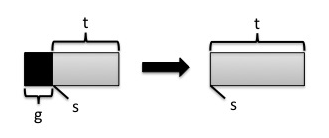
\includegraphics[scale=0.4]{./img/conversion}
	
\end{figure}

Além disso o conjunto $A$ contém apenas um tipo de arco, o arco do tipo 1 se os
voos satisfazem a restrição geográfica e o arco do tipo 3 caso não satisfaçam.
Os arcos dos tipos 2 e 4 são modelados a partir  da variável $\delta$ que tem
seu custo acrescentado na função objetivo.

Essa estratégia permite a redução de 3 arcos para cada voo, o que deixa o
modelo mais leve.

O calculo dos custos são feitos através de um pré-processamento, onde os arcos
viáveis recebem os valores referentes ao seu tipo, por exemplo, no caso de um
arco originário do nó origem, arco do tipo 6, um custo 1000 é atribuído. No
caso de arcos que deverão ser evitados um custo elevado é atribuído.
  	
  	
%\section{Pré-processmanto da instância}

%No caso da instância possuir mais de um dia de operação então pode-se quebra-la
%em dias se houver tempo vago entre os dias dessa instância.
  
\section{Fase de construção do GRASP}\label{sessao:construcao}
  
A construção da solução é feita elemento a elemento utilizando o
GRASP. Inicialmente é feita a ordenação do conjunto de voos a partir do seu
tempo de partida sugerido. O algoritmo só termina quando todos os voos já
foram alocados em algum trilho.
  
Existem duas formas de fazer a montagem da solução, uma seria a montagem de
trilhos de forma sequencial, onde um novo trilho só é iniciado quando o anterior
se encontra saturado. A outra forma é a montagem de trilhos de forma paralela,
que, a priori, provocaria uma melhor distribuição dos voos. Na prática a
primeira abordagem foi adotada, pois, nas instâncias disponíveis ela apresentou,
sempre, soluções de melhor qualidade. 

Pode ser que para instâncias com alguma característica específica a
estratégia de montagem dos trilhos de forma paralela pode apresentar melhores
resultados.


  
\subsection{Formação dos trilhos de forma sequencial}

Quando se pensa na escolha do primeiro voo do trilho, a decisão imediata é a
escolha do voo que contenha o menor horário de partida sugerido, ou seja, o voo
mais próximo. Porém essa escolha reduz a quantidade de soluções que podem ser
geradas, isso ocorre pois o primeiro voo tem uma grande influência nas
possíveis soluções que um trilho pode assumir. Para evitar isso a escolha do
primeiro voo de um trilho é feita baseando-se nos 5 voos com menor horário de
partida que ainda não estejam alocados a nenhum outro trilho. 

Esses voos são adicionados a lista de candidatos iniciais (LCI) em seguida é
feita a escolha do elemento que irá iniciar o novo trilho levando em
consideração apenas os elementos que possuam o horário de partida distante de
até $\alpha \%$ do voo de menor horário de partida, esses elementos são então
inseridos em uma lista restrita inicial (LCI) na qual é feita a seleção
aleatório de um dos voos. Isso é feito para evitar a escolha de um voo muito
distante do menor voo.

Os pseudocódigos \ref{alg:selectinit} e \ref{alg:formseq} ajudam a elucidar esse
entendimento. Primeiro deve-se entender o pseudocódigo \ref{alg:selectinit}
onde é feito a escolha de um voo que deverá iniciar um trilho, esse
pseudocódigo serve tando para montar trilhos de forma sequencial como de forma
paralela. Em 1 é formada a LCI que é composta pelos 5 primeiros voos ainda não
alocados, de 2 a 4 é feita a formação da LRI tendo como base o menor horário de
partida $h(v_{min})$, o maior horário de partida $h(v_{max})$ e o $\alpha$ e em
5 é feita a escolha aleatória de um desses voos. Já no pseudocódigo
\ref{alg:formseq} é feita a montagem dos trilhos de forma sequencial. Em 1 os
voos disponíveis são ordenados de acordo com seu horário de partida, em 2 a
malha, que será o resultado, é inicializada com vazio. De 3 a 9 é feita a
montagem dos trilhos que irão compor a malha, em 4 e 5 é obtido o primeiro voo
do trilho, em 6 é feita a montagem completa desse trilho, em 7 os voos
pertencente ao trilho corrente são removidos do conjunto de voos disponíveis e
em 8 o trilho corrente é adicionado a malha resultante.

 \begin{figure}[h]
\caption{Pseudocódigo do procedimento de seleção de um voo inicial. \newline
\mbox{Fonte: Própria}}\label{alg:selectinit}
\begin{programma}
\ALGORITHM{selecionaVooInicial(V)}

\STATE $LCI$ \GETS cincoPrimeirosVoos($V$);
\STATE $h(v_{min}) \GETS min\{h(v) \mid v \in LCI\}$;
\STATE $h(v_{max}) \GETS max\{h(v) \mid v \in LCI\}$;
\STATE $LRI \GETS \{v \in LCI \mid h(v) \leq h(v_{min}) + \alpha(h(v_{max}) -
h(v_{min}))\}$;
\STATE Selecione aleatoriamente um elemento $v \in LRI$;
\STATE\RETURN $v$;
\ENDALGORITHM
\end{programma}
\end{figure}

\begin{figure}[h]
\caption{Pseudocódigo do procedimento de formação sequencial dos trilhos.
\newline
\mbox{Fonte: Própria}}\label{alg:formseq}
\begin{programma}
\ALGORITHM{formaçãoSequencialDosTrilhos(V)}

\STATE Ordene o conjunto de voos não alocados $V$;
\STATE $M \GETS \emptyset$;
\WHILE{$V \neq \emptyset$}
\STATE $v \GETS selecionaVooInicial(V)$
\STATE $T \GETS \{v\}$;
\STATE $T \GETS completaTrilho(T)$;
\STATE $V \GETS V - \{v \in T\}$;
\STATE $M \GETS M \cup T$;
\ENDWHILE
\STATE\RETURN $M$;

\ENDALGORITHM
\end{programma}
\end{figure}


\subsection{Formação dos trilhos de forma paralela}
 
Nessa estratégia um trilho é iniciado sempre que existe um voo que não pode ser
inserido em nenhum dos trilhos que estejam sendo montados, mantendo-se assim um
conjunto de trilhos disponíveis (CTD).

Em cada iteração o trilho corrente (TC) é escolhido a partir do CTD de forma
aleatória. Feito isso, adiciona-se um voo a esse trilho. Caso não existam voos
candidatos para adição no TC este é removido da CTD e uma nova iteração é
iniciada.

O pseudocódigo \ref{alg:formparalel} ajudam no entendimento do algoritmo. Em 1
os voos disponíveis são ordenados de acordo com seu horário de partida, em 2 e 3
respectivamente a malha resultante e o CDT são inicializados com vazio. De 4 a
19 é feita a montagem paralela dos trilhos que irão formar a malha. Em 5 é feita
a seleção de um voo inicial. Em 6 verifica-se se existe algum trilho corrente
que pode incorporar esse voo, se existir então em 7 é feita a seleção de um
trilho corrente (TC) a partir dos elementos da CDT e em 8 seleciona-se um voo
que possa ser inserido em TC e insere o voo em 13. 	Se não existir nenhum
voo que possa ser inserido em TC então este é removido da CDT como pode ser
visto de 9 a 12. 

De 15 a 18 é criado um novo trilho sempre que não existe nenhum trilho da CDT
que possa comportar o voo selecionado em 5. Em 20 se insere os trilhos
pertencentes a CDT na malha resultante. Isso ocorre porque todos os voos já
foram alocados em algum trilho.



\begin{figure}[h]
\caption{Pseudocódigo do procedimento de formação paralela dos trilhos.
\newline
\mbox{Fonte: Própria}}\label{alg:formparalel}
\begin{programma}
\ALGORITHM{formaçãoParalelaDosTrilhos(V)}

\STATE Ordene o conjunto de voos não alocados $V$;
\STATE $M \GETS \emptyset$;
\STATE $CTD \GETS \emptyset$;
\WHILE{$V \neq \emptyset$}
\STATE $v \GETS selecionaVooInicial(V)$
\IF {$v$ pode ser inserido em um trilho do CTD}
	\STATE $TC \GETS escolheTrilhoAleatório(CTD)$;
	\STATE $nv \GETS selecionaVooCandidato(TC)$;
	\IF {$nv = \emptyset$}
		\STATE $CDT \GETS CDT - \{TC\}$
		\STATE $M \GETS M \cup \{TC\}$
	\ELSE
		\STATE $TC \GETS TC \cup \{nv\}$
	\ENDIF
\ELSE
	\STATE $T \GETS \{v\}$; 
	\STATE $CTD \GETS CTD \cup T$ 	
\ENDIF
\ENDWHILE

\STATE $M = M \cup \{t \in CTD\}$;
\STATE\RETURN $M$;

\ENDALGORITHM
\end{programma}
\end{figure}


  
\subsection{Escolha dos voos de um trilho}

A escolha do primeiro voo de um trilho é feita como explicado nas seções
anteriores enquanto os demais voos são escolhidos tendo como base um tipo de
arco e uma lista restrita de candidatos (CLR).
 
Os tipos de arcos foram definidos no Capítulo \ref{cap:descprob}, porém nessa
etapa apenas 4 tipos são considerados, o   $a_{1},a_{2},a_{3},a_{4}$ que
representam formas de ligações entre os voos. Os arcos do tipo 5 e 6 só são
utilizados na modelagem matemática. Os arcos do tipo 1 permitem a
ligação de voos sem a utilização de atrasos e/ou reposicionamentos. Os arcos do
tipo 2 utilizam atrasos mas não o reposicionamento. Os arcos do tipo 3 permitem
o sequenciamento com a utilização de um voo de reposicionamento mas sem inserir
atraso em nenhum dos voos envolvidos. Os arcos do tipo 4 utilizam-se de atrasos
e de um voo de reposicionamento para fazer a ligação entre dois voos. Os arcos
do tipo 5 pargem do nó \textit{source} e servem para modelar o inicio de um
trilho. Os arcos do tipo 6 tem chegam ao nó \textit{sink} e indicam o fim de um
trilho.

Primeiramente é feita a escolha do tipo de arco que será utilizado para efetuar
a ligação do ultimo voo do trilho corrente. Essa escolha é feita tendo
como base as probabilidades de cada um desses arcos acontecer. Essa
probabilidade foi definida como sendo
$P(a_{1})=0.79,P(a_{2})=0.16,P(a_{3})=0.04,P(a_{4})=0.01$ pois a solução ótima
do problema real da Rio Sul apresentava essas características. Esses valores
são empíricos e para determinadas instâncias podem gerar melhores soluções se
alterados.

De posse do tipo de arco, é feita então a formação da lista de candidatos. Essa
lista é ordenada de acordo com o seu horário de partida sugerido, caso o arco
seja do tipo $A_{1}$, ou pelo custo associado a sua escolha para os demais
tipos de arco. No caso da lista de candidatos não possuir nenhum voo, então
outro tipo de arco é sorteado, até que não seja possível acrescentar voos ao
trilho de nenhuma forma, quando isso ocorrer a construção
desse trilho é finalizada.
 
Caso seja possível a obtenção de uma lista de candidatos então ela é reduzida
tendo como base o passo 4 a 6 do algoritmo \ref{alg:graspcons} formando assim a
lista de candidatos restrita (LCR), essa redução remove os candidatos que estão
muito afastado do melhor candidato da lista. Como está lista se encontra
ordenada, então, o elemento de menor impacto ($v_{menor}$) na solução é o
primeiro e o de maior impacto ($v_{maior}$) é o último. A LCR contém os
candidatos que tenha o valor de impacto na solução de até $valor_{menor} +
\alpha*(valor_{maior} + valor_{menor})$, onde $\alpha$ é o grau de
gulosidade do GRASP. O candidato deve ser escolhido de forma aleatória entre os
elementos da LCR.

O pseudocódigo \ref{alg:calcvoo} explica como isso acontece. Em 1 inicializa o
conjunto de arcos com os 4 tipos possíveis em 2 realiza-se um sorteio do tipo de
arco que irá ser inicialmente avaliado levando em consideração a probabilidade
de cada um deles acontecer ($P(a_{1}), P(a_{2}), P(a_{3}), P(a_{4})$). Em 3 é
feita a remoção do tipo de arco selecionado do conjunto inicial e em 4
é selecionado o voo corrente que necessita de um sucessor, nesse caso o último
voo do trilho.

De 5 a 13 procura-se um candidato para o voo corrente levando em consideração
todos os tipos de arcos, iniciando pelo que foi selecionado no passo 2.

\begin{figure}[h]
\caption{Pseudocódigo de calculo do proximo voo de um trilho
\newline
\mbox{Fonte: Própria}}\label{alg:calcvoo}
\begin{programma}
\ALGORITHM{obtemProximoVoo(T,V)}

\STATE $A \GETS \{1,2,3,4\}$;
\STATE $a \GETS sorteaTipoDeArco(A, P(a_{1}),P(a_{2}),P(a_{3}),P(a_{4}))$;
\STATE $A \GETS A - \{a\}$; \STATE $v \GETS ultimoVoo(T)$;

\FOR{$i$ \FROM $1$ \TO $4$}\PGlnlabel{forline}
\STATE $c \GETS proximoCandidato(v, V, a)$;
\IF {$c = \emptyset$}
	\STATE $a \GETS proximoArco(A)$;
	\STATE $A \GETS A - \{a\}$;
\ELSE
	\STATE\RETURN $c$;
\ENDIF 
\ENDFOR

\STATE\RETURN $\emptyset$;

\ENDALGORITHM
\end{programma}
\end{figure}
 
 \section{Fase de busca local do GRASP}

Com a finalização da etapa anterior tem-se uma solução do problema. A fase de busca
local efetua modificações nessa solução com a finalidade de obter outras
melhores que estejam próximos a ela, isso é feito através da aplicação das
estruturas de vizinhanças. No método proposto essa fase foi implementada através
da utilização da metaheurística ILS que alterna busca local com pertubações
conseguindo assim escapar de mínimos locais quando não consegue mais melhorar a
solução, ou seja, primeiro são aplicados as estruturas de vizinhança, visando
obter o valor ótimo local da solução, depois é feita uma perturbação que
diversifica melhorando o valor da função objetivo através da aplicação do
modelo matemático que foi desenvolvido em uma parte do problema. Quando nenhuma
das duas estratégias consegue melhorar a solução então a busca local encerra e
uma nova iteração do GRASP pode ser iniciada.
 
\subsection{Estruturas de vizinhança}
 
Foram definidas três estruturas de vizinhança para serem utilizadas na busca
local, o Swap-X e o Cross-Over, que tem o objetivo de remover modificações nos
horários de partida sugeridos dos voos, e a Compactação, que promove a redução
do número de trilhos. Abaixo essa estruturas são explicadas.
 
\subsubsection{Swap-X}

Esse operador efetua a troca de X voos de um trilho por um conjunto de voos de
outro trilho. Dessa forma pode-se conseguir remover os atrasos que foram criados
na etapa de construção. No método proposto apenas os movimentos do tipo Swap-1
e Swap-2 são utilizados, pois essa vizinhança é considerada grande. Na Figura
\ref{fig:swap1} um caso de melhoria no custo dos trilhos é exemplificada.

\begin{figure}[ht]
	\caption{Estrutura de vizinhança Swap-1. \newline \mbox{Fonte:
	(Própria)}}\label{fig:swap1}
	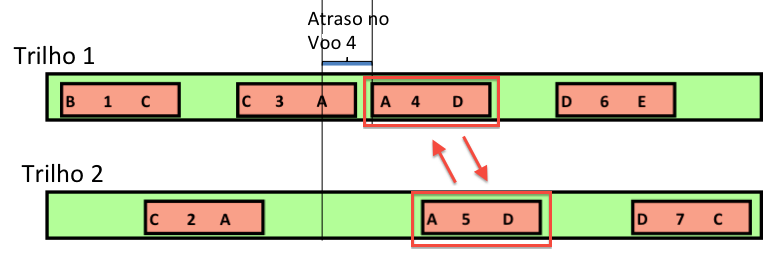
\includegraphics[scale=0.4]{./img/swap-1}
	
\end{figure}
 
 \subsubsection{Cross-Over}
 
A ideia do operador $crossover$ é a de efetuar troca entre dois segmentos de
trilhos com a finalidade de gerar novos trilhos com menos modificações no
horário de partida. A Figura \ref{fig:crossover} ilustra uma melhoria causada por um
movimento desse tipo.


\begin{figure}[ht]
	\caption{Estrutura de vizinhança CrossOver. \newline \mbox{Fonte:
	(Própria)}}\label{fig:crossover}
	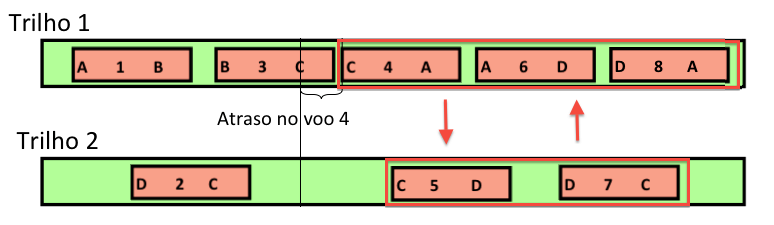
\includegraphics[scale=0.4]{./img/crossover}
	
\end{figure}
 
 \subsubsection{Compactação}
 
A compactação é a única estrutura de vizinhança utilizada que é capaz de
reduzir a quantidade de trilhos da solução final.
 
Isso ocorre porque ela consegue, insere um trilho em outro de forma direta ou
com a utilização de um voo de reposicionamento.
 
A figura \ref{fig:compactacao} mostra a redução de um trilho com a utilização
desse movimento.

\begin{figure}[ht] 
	\caption{Estrutura de vizinhança Compactação. \newline \mbox{Fonte:
	(Própria)}}\label{fig:compactacao}
	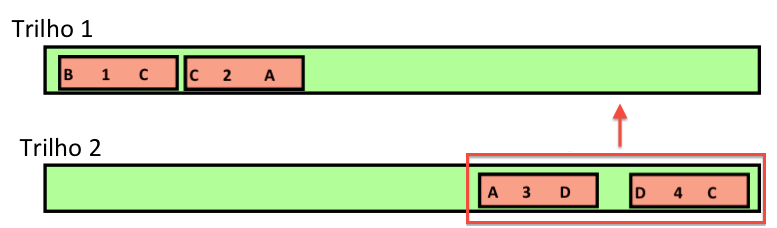
\includegraphics[scale=0.4]{./img/compactacao}
	
\end{figure}
 
 \subsection{Perturbação usando o método exato}
   
A perturbação normalmente é utilizada quando as estruturas de vizinhança não
conseguem melhorar a solução, quando isso ocorre, pode-se dizer que a
solução corrente é a ótima local com relação a vizinhança que foi definida.
 
Para tentar encontrar outros mínimos locais aplica-se uma modificação na
estrutura da solução, mesmo que isso provoque uma piora na sua qualidade. Isso
se mostra interessante para o algoritmo pois ele irá efetuar busca de melhorias
em outros locais no espaço de soluções através da sua busca local.
 
O método de perturbação utilizado aqui difere do que normalmente é aplicado
pois a solução tem a sua estrutura modificada e ainda consegue melhorar a sua
qualidade. Isso é feito através da aplicação do modelo matemático em uma
parte do problema. A sua utilização ocorre com a seleção de um conjunto de
trilhos, e sua a posterior aplicação no solver com o modelo desenvolvido
configurado para o conjunto de voos da seleção.

O método exato retorna a configuração ótima desses voos, que
são agrupados novamente a solução antiga. O solver tem um tempo máximo
estabelecido e se não retornar nenhuma solução considera-se que não houve
melhora sua aplicação.

A seleção dos trilhos é feita com base no seu
\textit{grau de compactação} que é definido como sendo porcentagem de
utilização efetiva de um trilho com relação ao tempo de partida do primeiro voo
e o tempo de chegada do último voo da instância, ou seja, quanto maior o tempo
que a aeronave, que opera um determinado trilho, permanece voando maior será o
seu grau de compactação. O calculo do grau de compactação não leva em
consideração os voos de reposicionamento, pois eles não estão no planejamento
inicial e por sua vez não são passados para o modelo.

Existe três formas de fazer a seleção dos trilhos que serão aplicados no solver,
pode-se adicionar os trilhos que possuem o maior grau de compactação, pode-se
adicionar os trilhos que possuem o menor grau de compactação ou pode-se alternar
entre a escolha de um trilho com o maior grau de compactação e um de menor grau
de compactação.

Na prática adotou-se a segunda abordagem, selecionando os trilhos de menor grau
de compactação, pois os resultados foram melhores.
 
Os trilhos são adicionados a solução até o limite de 80 voos, pois o solver
conseguiu em nossos experimentos resolver um problema desse porte de forma
imediata. 

\subsection{Método de construção paralela}

A estratégia paralela foi desenvolvida para aumentar a escalabilidade na
resolução de grandes problemas e também na tentativa de obter melhores soluções
em um menor espaço de tempo. O seu funcionamento parte da divisão da instância
em períodos de tempos iguais que são distribuídas para cada processo. Em cada
período os processos realizam uma construção do algoritmo descrito na sessão
\ref{sessao:construcao}. Ao final dessa etapa cada processo possui um um
conjunto de trilhos que devem ser ligados uns com os outros para a geração de
uma malha de voo completa.
 
O algoritmo é dividido em passos onde em cada passo um
nível diferente de vizinho é visitado na tentativa de efetuar a ligação dos seus
trilhos. No nível 1 é feita a comunicação seguindo a topologia de uma
rede em anel, onde cada processo fala com seu vizinho sucessor a uma distância
de 1, ou seja, o processo 0 fala com o processo 1, o 1 com o 2 e assim por
diante até que o último processo fale com o processo 0. Quando todos as tentativas de
ligação de trilhos entre esses processo são esgotados então o passo do algoritmo
é incrementado para que o processo consiga conversar com o processo sucessor que
possua uma distância de 2 dele, ou seja, o processo 0 se comunica com o processo
2, o 1 com o 3 e assim por diante, isso ocorre até que todos os processo tenham
se comunicados com os outros ou até que todos os trilhos estejam ligados.

Essa estratégia é interessante pois normalmente as empresas trabalham com uma
malha circular que costuma se repetir toda a semana.

O pseudocódigo \ref{alg:metodoparalel} simplifica o entendimento do algoritmo.
Perceba que a complexidade de execução e de mensagens do algoritmo distribuído
\ref{alg:metodoparalel} no pior caso é de $O(s.c)$, onde $s$ é o número de
processos e $c$ é a maior quantidade de trilhos de um processo.


\begin{figure}[h]
\caption{Pseudocódigo do método de comunicação paralela usado na construção dos
trilhos.
\newline
\mbox{Fonte: Própria}}\label{alg:metodoparalel}
\begin{programma}
\ALGORITHM{inicioComunicacaoParalela(M, s, r)}

\STATE inicializaVoos(M,s,r);
\FOR{$cn$ \FROM $1$ \TO $(s-1)$}\PGlnlabel{forline}
\STATE $dest \GETS (r + cn)$ MOD $s$;
\STATE $c \GETS 0$;
\FOREACH{$t$ \IN $M$}
\STATE $f \GETS ultimoVoo(t)$;
	\IF{f ainda não foi selecionado}
	\STATE $c \GETS c + 1$;
	\STATE solicitaConexão(f, dest);
	\ENDIF
\ENDFOR

\STATE EnviaFinalizaMsg(dest);

\WHILE{Não tiver respondido todas as requisições}
	\STATE $P \GETS RecebeMSG()$;
	\IF{P é uma solicitação de conexão}
		\STATE $f \GETS $selecionaUmVoo(M, P.voo);
		\IF{$f \neq \emptyset$}
			\STATE EfetuaConexão(P, f);
		\ELSE
			\STATE RejeitaConexão(P, f);
		\ENDIF
	\ELSEIF{P é uma aceitação de conexão}
		\STATE ConfiguraLigação(P);
	\ELSEIF{P é uma finalização de mensagens}
		\STATE $F \GETS verdadeiro$;
	\ENDIF 
	
\ENDWHILE
\ENDFOR

\ENDALGORITHM
\end{programma}
\end{figure} 


A linha 1 é utilizada na inicialização dos voos, onde cada processo obtém o
conjunto de voos que irá trabalhar, esse conjunto de voos é definido pela
instância $M$, pelo número de processor que estão executando $s$ e pelo número
do processo corrente $r$. O laço iniciado na linha 2 modela a quantidade de
iterações do algoritmo, que é baseado no número de processos. A variável $cn$ é
o contador de nível e informa para qual vizinho o processo corrente irá tentar
efetuar ligações dos seus trilhos disponíveis.

O cálculo do índice do processo que irá receber a comunicação é feita na linha
3. A linha 4 inicia o contador de mensagens enviadas, que é usado como auxiliar
de condição de parada no laço da linha 13.

É feito então uma tentativa de conectar os trilhos que ainda não
foram conectados com os trilhos dos vizinhos. Nas linhas 6 a 10 é
feito o envio de solicitações de conexões de todos os últimos voos ainda não
conectados de cada um dos seus trilhos para o vizinho corrente que é definido
pela variável $dest$. Na linha 12 o processo sinaliza para o seu vizinho
corrente que não tem mais nenhum trilho para tentar efetuar uma ligação.

Depois o processo passa a agir como uma máquina de estados, como pode ser visto
nas linhas 13 a 27, respondendo as requisições que forem recebendo. Isso
acontece até ele receber uma mensagem de finalização do seu vizinho e todas as mensagens
que ele tenha enviado anteriormente tenham sido respondidas. Na linha 14
o processo recebe uma mensagem que vai lhe informar qual a ação que deverá
ser executada.

Quando a mensagem é uma solicitação de conexão, linhas 15 a 22, então o processo
tenta selecionar um voo, do inicio de um de seus trilhos, que ainda não tenha se
ligado com nenhum outro trilho para se ligar com o voo candidato da solicitação.
A escolha do voo que vai se ligar é feita usando o GRASP com uma LRC. Caso
exista algum voo que possa se conectar, linha 17, então uma mensagem de
aceitação de conexão é enviada para o solicitante e o voo é marcado como já
selecionado, isso é feito no procedimento \textit{EfetuaConexão(P, f)}. Caso
não exista nenhum voo que possa se candidatar então uma mensagem de rejeição de
conexão é enviada pelo procedimento \textit{RejeitaConexão(P, f)}.

As linhas 22 a 24 é executada quando o processo recebe uma mensagem de aceitação
ou rejeição de conexão e é utilizada para configurar o voo que teve a
solicitação aceita. Já as linhas 24 a 26 marca a flag de finalização do vizinho
$F$ como verdadeiro.

Na prática essa estratégia conseguiu obter resultados aproximadamente 10\%
melhores que a estratégia sequencial, ou seja, de um processo com a fatia
completa do tempo, levando em consideração apenas a fase de construção. Por
questões de tempo esse experimento não foi concluído, com a inserção da fase de
refinamento que utiliza o \textit{solver}.

Para justificar o uso de uma estratégia mais eficiente, como essa, seria
necessário obter primeiro uma instância que não obtivesse resultados
satisfatórios com a estratégia híbrida sequencial. Aparentemente essa nova
estratégia iria ocasionar melhoras nos resultados finais já que a qualidade da
solução gerada na construção tem influencia direta na velocidade que o
algoritmo encontra uma melhor solução.



% Dessa forma o
%número de processos que serão usados deverá ser calibrado de acordo com a
%duração da instância.

%Nos testes realizados constatou-se que fatias de tempos menores que 6 horas não
% conseguiram gerar resultados satisfatórios.
 
 